% Options for packages loaded elsewhere
\PassOptionsToPackage{unicode}{hyperref}
\PassOptionsToPackage{hyphens}{url}
%
\documentclass[
  english,
  man,floatsintext]{apa7}
\usepackage{lmodern}
\usepackage{amssymb,amsmath}
\usepackage{ifxetex,ifluatex}
\ifnum 0\ifxetex 1\fi\ifluatex 1\fi=0 % if pdftex
  \usepackage[T1]{fontenc}
  \usepackage[utf8]{inputenc}
  \usepackage{textcomp} % provide euro and other symbols
\else % if luatex or xetex
  \usepackage{unicode-math}
  \defaultfontfeatures{Scale=MatchLowercase}
  \defaultfontfeatures[\rmfamily]{Ligatures=TeX,Scale=1}
\fi
% Use upquote if available, for straight quotes in verbatim environments
\IfFileExists{upquote.sty}{\usepackage{upquote}}{}
\IfFileExists{microtype.sty}{% use microtype if available
  \usepackage[]{microtype}
  \UseMicrotypeSet[protrusion]{basicmath} % disable protrusion for tt fonts
}{}
\makeatletter
\@ifundefined{KOMAClassName}{% if non-KOMA class
  \IfFileExists{parskip.sty}{%
    \usepackage{parskip}
  }{% else
    \setlength{\parindent}{0pt}
    \setlength{\parskip}{6pt plus 2pt minus 1pt}}
}{% if KOMA class
  \KOMAoptions{parskip=half}}
\makeatother
\usepackage{xcolor}
\IfFileExists{xurl.sty}{\usepackage{xurl}}{} % add URL line breaks if available
\IfFileExists{bookmark.sty}{\usepackage{bookmark}}{\usepackage{hyperref}}
\hypersetup{
  pdftitle={Dependency learning: comparing adults and children},
  pdflang={en-EN},
  hidelinks,
  pdfcreator={LaTeX via pandoc}}
\urlstyle{same} % disable monospaced font for URLs
\usepackage{graphicx}
\makeatletter
\def\maxwidth{\ifdim\Gin@nat@width>\linewidth\linewidth\else\Gin@nat@width\fi}
\def\maxheight{\ifdim\Gin@nat@height>\textheight\textheight\else\Gin@nat@height\fi}
\makeatother
% Scale images if necessary, so that they will not overflow the page
% margins by default, and it is still possible to overwrite the defaults
% using explicit options in \includegraphics[width, height, ...]{}
\setkeys{Gin}{width=\maxwidth,height=\maxheight,keepaspectratio}
% Set default figure placement to htbp
\makeatletter
\def\fps@figure{htbp}
\makeatother
\setlength{\emergencystretch}{3em} % prevent overfull lines
\providecommand{\tightlist}{%
  \setlength{\itemsep}{0pt}\setlength{\parskip}{0pt}}
\setcounter{secnumdepth}{-\maxdimen} % remove section numbering
% Make \paragraph and \subparagraph free-standing
\ifx\paragraph\undefined\else
  \let\oldparagraph\paragraph
  \renewcommand{\paragraph}[1]{\oldparagraph{#1}\mbox{}}
\fi
\ifx\subparagraph\undefined\else
  \let\oldsubparagraph\subparagraph
  \renewcommand{\subparagraph}[1]{\oldsubparagraph{#1}\mbox{}}
\fi
% Manuscript styling
\usepackage{upgreek}
\captionsetup{font=singlespacing,justification=justified}

% Table formatting
\usepackage{longtable}
\usepackage{lscape}
% \usepackage[counterclockwise]{rotating}   % Landscape page setup for large tables
\usepackage{multirow}		% Table styling
\usepackage{tabularx}		% Control Column width
\usepackage[flushleft]{threeparttable}	% Allows for three part tables with a specified notes section
\usepackage{threeparttablex}            % Lets threeparttable work with longtable

% Create new environments so endfloat can handle them
% \newenvironment{ltable}
%   {\begin{landscape}\begin{center}\begin{threeparttable}}
%   {\end{threeparttable}\end{center}\end{landscape}}
\newenvironment{lltable}{\begin{landscape}\begin{center}\begin{ThreePartTable}}{\end{ThreePartTable}\end{center}\end{landscape}}

% Enables adjusting longtable caption width to table width
% Solution found at http://golatex.de/longtable-mit-caption-so-breit-wie-die-tabelle-t15767.html
\makeatletter
\newcommand\LastLTentrywidth{1em}
\newlength\longtablewidth
\setlength{\longtablewidth}{1in}
\newcommand{\getlongtablewidth}{\begingroup \ifcsname LT@\roman{LT@tables}\endcsname \global\longtablewidth=0pt \renewcommand{\LT@entry}[2]{\global\advance\longtablewidth by ##2\relax\gdef\LastLTentrywidth{##2}}\@nameuse{LT@\roman{LT@tables}} \fi \endgroup}

% \setlength{\parindent}{0.5in}
% \setlength{\parskip}{0pt plus 0pt minus 0pt}

% \usepackage{etoolbox}
\makeatletter
\patchcmd{\HyOrg@maketitle}
  {\section{\normalfont\normalsize\abstractname}}
  {\section*{\normalfont\normalsize\abstractname}}
  {}{\typeout{Failed to patch abstract.}}
\makeatother
\shorttitle{Dependency learning}
\author{Jens Roeser\textsuperscript{1}}
\affiliation{
\vspace{0.5cm}
\textsuperscript{1} Department of Psychology, Nottingham Trent University, United Kingdom}
\authornote{

Correspondence concerning this article should be addressed to Jens Roeser, 50 Shakespeare St, Nottingham NG1 4FQ. E-mail: jens.roeser@ntu.ac.uk}
\keywords{}
\usepackage{csquotes}
\usepackage{booktabs}
\usepackage{longtable}
\usepackage{graphicx}
\usepackage{array}
\usepackage{float}
\usepackage{threeparttable}
\usepackage[normalem]{ulem}
\usepackage[utf8]{inputenc}
\usepackage{icomma}
\ifxetex
  % Load polyglossia as late as possible: uses bidi with RTL langages (e.g. Hebrew, Arabic)
  \usepackage{polyglossia}
  \setmainlanguage[]{english}
\else
  \usepackage[shorthands=off,main=english]{babel}
\fi
\ifluatex
  \usepackage{selnolig}  % disable illegal ligatures
\fi
\newlength{\cslhangindent}
\setlength{\cslhangindent}{1.5em}
\newenvironment{cslreferences}%
  {\setlength{\parindent}{0pt}%
  \everypar{\setlength{\hangindent}{\cslhangindent}}\ignorespaces}%
  {\par}

\title{Dependency learning: comparing adults and children}

\date{}

\begin{document}
\maketitle

\hypertarget{comparisons-between-children-and-adults}{%
\section{Comparisons between children and adults}\label{comparisons-between-children-and-adults}}

In this final analysis we evaluate differences between the adults (Experiment 1) and the children results (Experiment 2). In particular, we focused on the effect of main interest to evaluate implicit learning; i.e.~the slowdown in reaction times in the transfer block (Block 7) relative to Block 6. To compared the data from adults and children we pooled the serial reaction-time data from both experiments and extracted the data from Block 6 and 7. This analysis was largely similar to the reaction-time models reported earlier: reaction times were modelled in Bayesian linear mixed-effects models. Reaction times for elements that were not part of an adjacent or nonadjacent dependency were included in the model as baseline. Model predictors were Age Group (levels: adults, children), Dependency (levels: dependency, baseline), Adjacency (levels: adjacent, nonadjacent), Block (levels: 6, 7), and all by-Dependency and by-Adjacency interactions. All predictors were sum-coded.

Reaction time data were fitted with a shifted-lognormal distribution, random intercepts for each stimulus image, and random participants intercepts and by-participant slow adjustments for all main effects and interactions. In additional to the parameter estimates as in the previous results section, we calculated from the posterior the standardised effect sizes \(\delta\), defined as \(\delta = \frac{\mu}{\sigma}\) , where \(\mu\) is the estimated parameter value of the effect of interest and \(\sigma\) is the pooled standard deviation. The effect size was calculated to allow comparisons across age group (Wagenmakers et al., 2010). For the effect sizes, we determined the region of practical equivalence (henceforth, ROPE) to assess the uncertainty of the effect size (Makowski et al., 2019). The ROPE is a range of values that are practically equivalent to a null effect (see e.g.~Kruschke, 2010, 2011). For the effect size we set the ROPE to be -0.1 and 0.1 (Kruschke, 2018) which is the range of negligible effects sizes (Cohn, 1988). The value returned is the amount of posterior samples (of the effect size) that fell inside the ROPE. A meaningful effect size should have no or a small proportion of posterior samples within the ROPE. In other words, the ROPE value indicates to what extent the posterior cannot rule out an negligible effect.

Table \ref{tab:tablemodel} summaries the model outcome for the serial reaction-time data. We found compelling evidence for longer reaction times for children compared to adults. Reaction times for Block 7 were longer than for Block 6. Further evidence was found for the two-way interactions of Age Group and Block, and Age Group and Dependency. Importantly, we found evidence for the three-way interaction for both Dependency and Adjacency by Block and Age Group.

\begin{table}[ht]

\begin{center}
\begin{threeparttable}

\caption{\label{tab:tablemodel}Age group comparison for serial reaction-time data. Shown are the estimated parameter values $\hat{\mu}$ (in msecs) and the effect size $\hat{\delta}$ for main effects and interactions of Age Group (levels: adults, children), Dependency (levels: dependency, baseline), Adjacency (levels: adjacent, nonadjacent).}

\begin{tabular}{lrrrrrr}
\toprule
 & \multicolumn{3}{c}{Parameter estimate} & \multicolumn{3}{c}{Effect size} \\
\cmidrule(r){2-4} \cmidrule(r){5-7}
Predictor & \multicolumn{1}{c}{$\hat{\mu}$} & \multicolumn{1}{c}{95\% HPDI} & \multicolumn{1}{c}{$P(\hat{\mu}<0)$} & \multicolumn{1}{c}{$\hat{\delta}$} & \multicolumn{1}{c}{95\% HPDI} & \multicolumn{1}{c}{ROPE}\\
\midrule
Main effects &  &  &  &  &  & \\
\ \ \ Age Group & -347 & [-408, -280] & >.999 & -5.4 & [-6.69, -4.21] & 0\%\\
\ \ \ Dependency & 6 & [-32, 43] & .404 & 0.08 & [-0.4, 0.56] & 35\%\\
\ \ \ Adjacency & -9 & [-38, 23] & .681 & -0.12 & [-0.5, 0.28] & 38\%\\
\ \ \ Block & -70 & [-108, -38] & >.999 & -0.92 & [-1.47, -0.51] & 0\%\\
Interactions &  &  &  &  &  & \\
\ \ \ Dependency $\times$ Block & -42 & [-86, 0] & .974 & -0.56 & [-1.15, 0] & 1\%\\
\ \ \ Adjacency $\times$ Block & -9 & [-41, 20] & .767 & -0.11 & [-0.53, 0.27] & 33\%\\
\ \ \ Age $\times$ Block & -67 & [-99, -36] & >.999 & -0.9 & [-1.33, -0.46] & 0\%\\
\ \ \ Age $\times$ Dependency & -64 & [-94, -34] & >.999 & -0.85 & [-1.26, -0.44] & 0\%\\
\ \ \ Age $\times$ Adjacency & -16 & [-42, 13] & .853 & -0.2 & [-0.56, 0.16] & 27\%\\
\ \ \ Dependency $\times$ Block $\times$ Age & -40 & [-72, -5] & .987 & -0.51 & [-0.95, -0.06] & 0\%\\
\ \ \ Adjacency $\times$ Block $\times$ Age & 55 & [20, 91] & <.001 & 0.69 & [0.27, 1.12] & 0\%\\
\bottomrule
\addlinespace
\end{tabular}

\begin{tablenotes}[para]
\normalsize{\textit{Note.} $\hat{\mu}$ = most probable parameter value; 95\% HPDI = interval containing 95\% of the probability mass; $P(\hat{\mu}<0)$ = probability of the true parameter value being smaller than 0; $\hat{\delta}$ = most probable effect-size estimate; ROPE = region of practical equivalence.}
\end{tablenotes}

\end{threeparttable}
\end{center}

\end{table}

Figure \ref{fig:plotgroupcomp} illustrates the modelled serial reaction-time data comparing the slowdown from Block 6 to Block 7 for the adult and the children group. The slowdown from Block 6 to 7 was tested within Age Group and Dependency / Adjacency to gain further insight into the source of the two three-way interactions. Reported are the effect sizes for each comparison.

\begin{figure}[ht]

{\centering 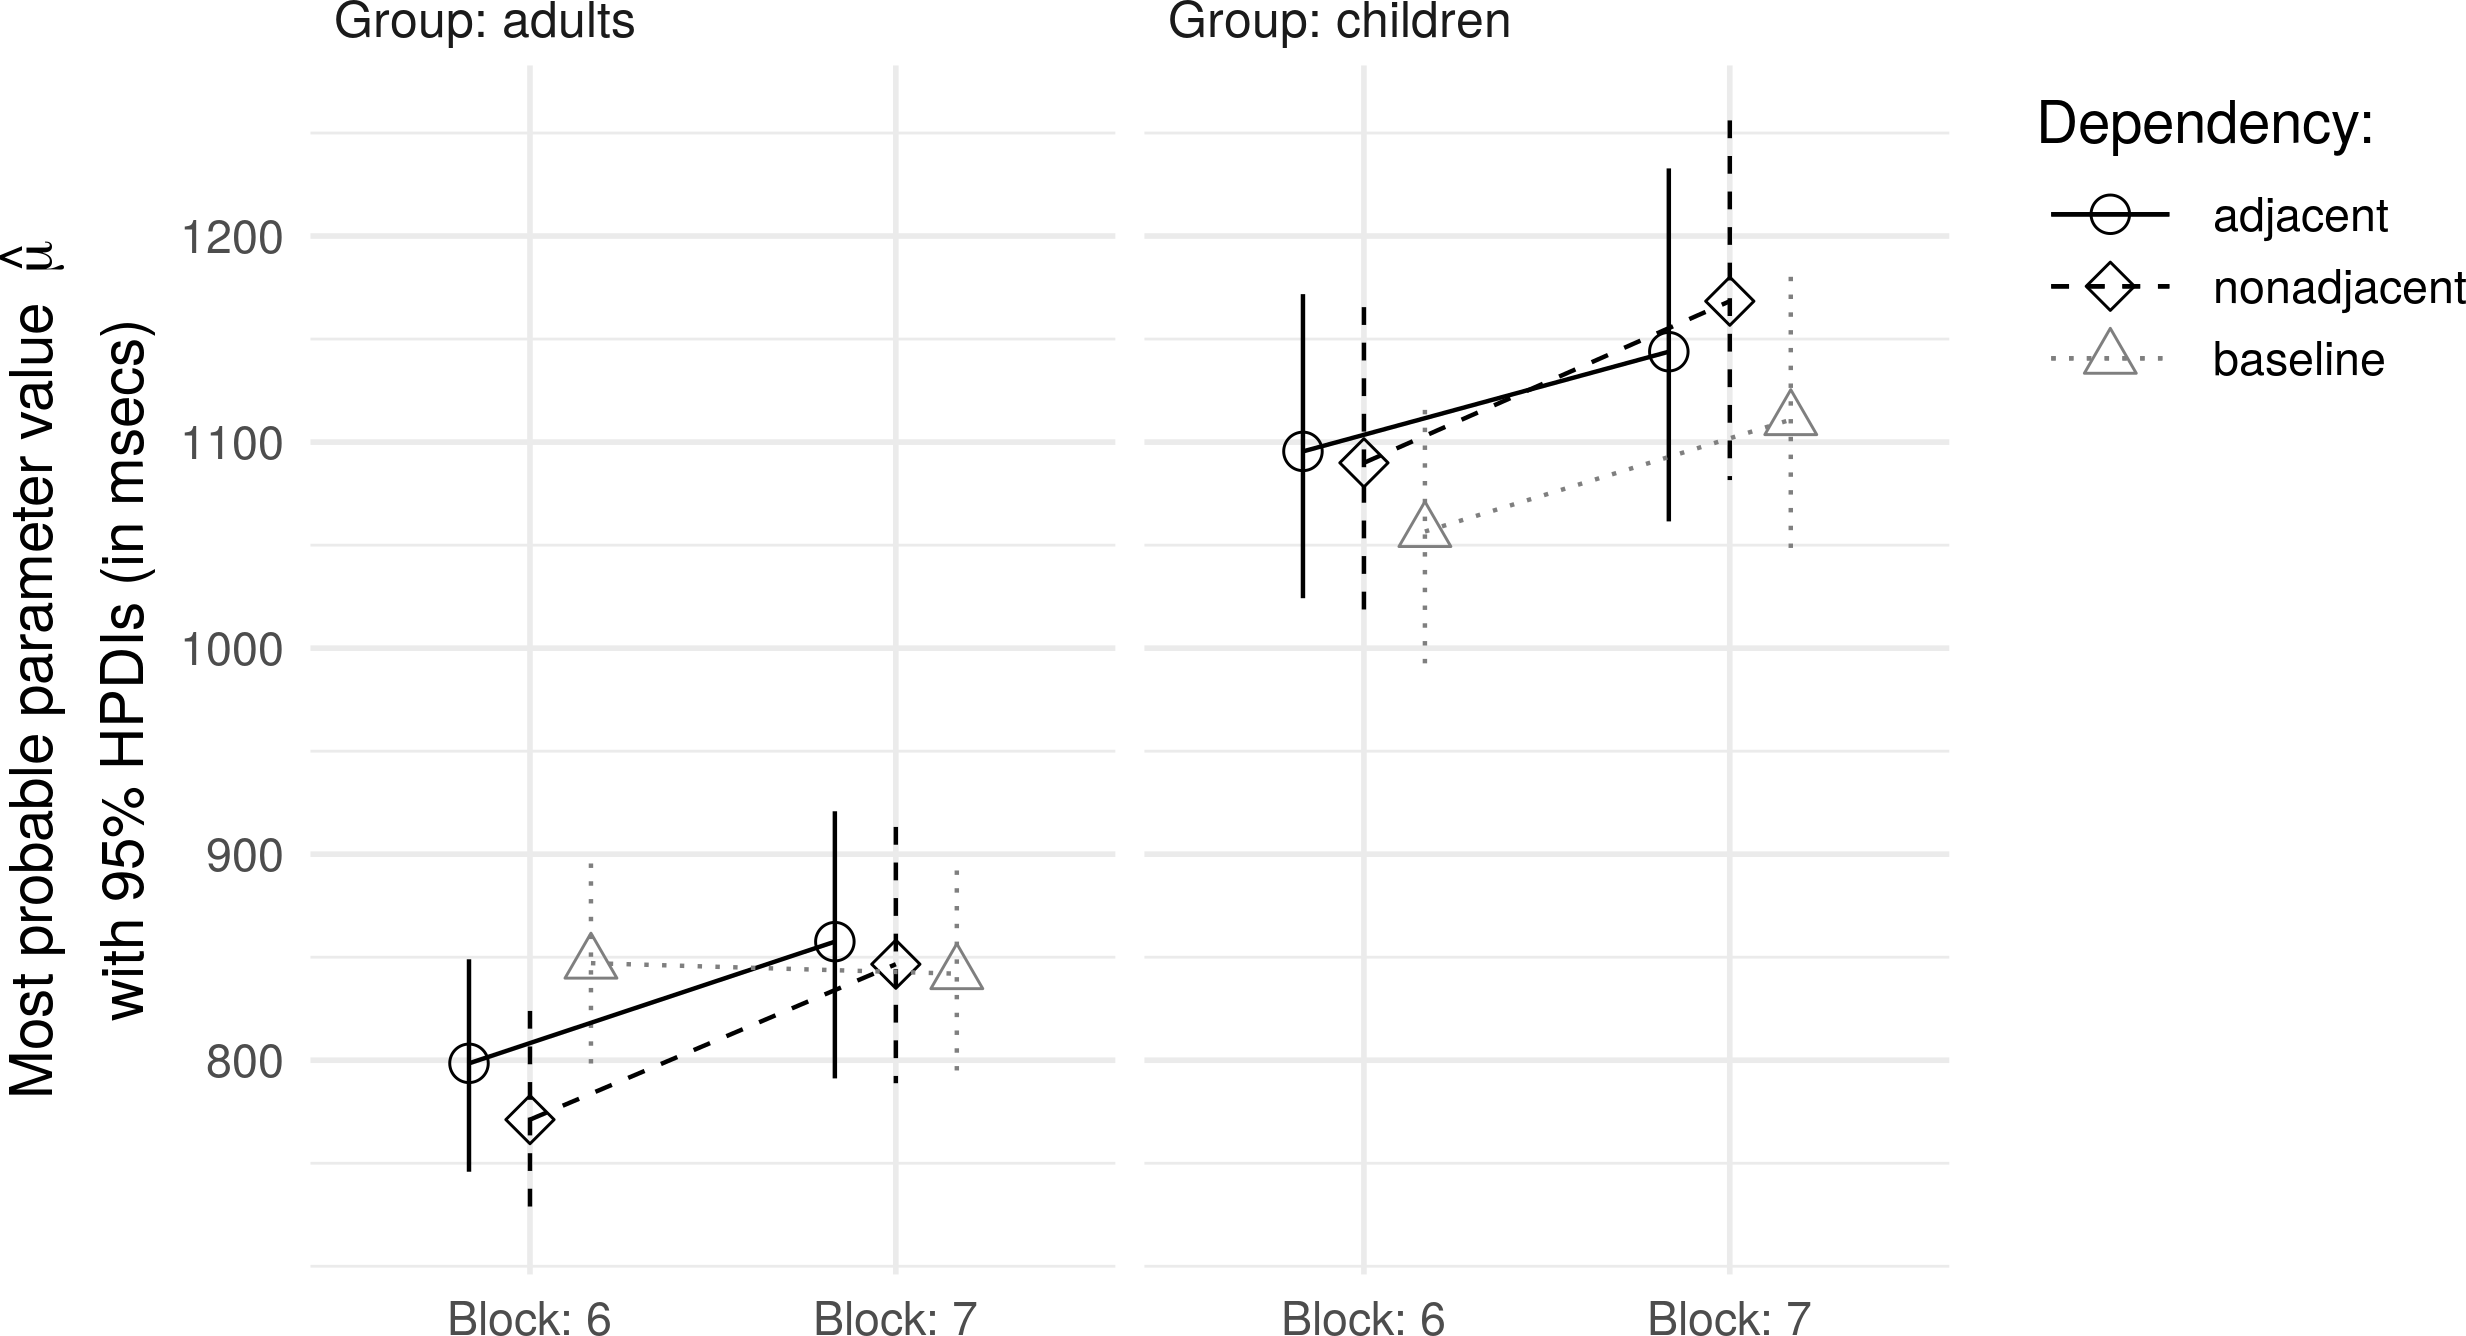
\includegraphics{Group-comparison_files/figure-latex/plotgroupcomp-1} 

}

\caption{Modelled serial reaction-time data (group comparison). Reaction time data for each age group for the final two blocks (block 7 is the transfer block). Shown are the modelled reaction-time data with 95\% HPDI (in msecs) for each dependency and adjacency type.}\label{fig:plotgroupcomp}
\end{figure}

First, we observed an interaction of Dependency (levels: dependency, baseline), Block, and Age Group. For the adult group, we observed a small effect for a slowdown from Block 6 to 7 in the dependency condition (\(\hat{\delta}\) = 0.23, 95\% HPDI{[}0.10, 0.40{]}, ROPE = 0\%) but negligible evidence for a slowdown in baseline trials (\(\hat{\delta}\) = -0.03, 95\% HPDI{[}-0.10, 0.08{]}, ROPE = 100\%). For the children group, we observed small slowdown effects in both the dependency condition (\(\hat{\delta}\) = 0.18, 95\% HPDI{[}0.01, 0.32{]}, ROPE = 13\%) and for the baseline condition (\(\hat{\delta}\) = 0.15, 95\% HPDI{[}0.03, 0.27{]}, ROPE = 14\%).

Second, we observed an interaction of Adjacency (levels: adjacent, nonadjacent), Block, and Age Group. Slowdown effects were found in adults for both adjacent (\(\hat{\delta}\) = 0.22, 95\% HPDI{[}0.01, 0.42{]}, ROPE = 8\%) and nonadjacent dependencies (\(\hat{\delta}\) = 0.28, 95\% HPDI{[}0.10, 0.48{]}, ROPE = 0\%). However, for the children group we observed a weak slowdown effect for adjacent dependencies that did not rule out the absence of an effect (\(\hat{\delta}\) = 0.13, 95\% HPDI{[}-0.07, 0.35{]}, ROPE = 35\%). The slowdown effect for nonadjacent dependencies was small (\(\hat{\delta}\) = 0.21, 95\% HPDI{[}0, 0.42{]}, ROPE = 10\%).

\newpage

\hypertarget{references}{%
\section{References}\label{references}}

\begingroup
\setlength{\parindent}{-0.5in}
\setlength{\leftskip}{0.5in}

\hypertarget{ref}{}

\endgroup

\hypertarget{refs}{}
\begin{cslreferences}
\leavevmode\hypertarget{ref-cohn1988statistical}{}%
Cohn, J. (1988). \emph{Statistical power analysis for the behavioral sciences}. Lawrence Earlbam Associates.

\leavevmode\hypertarget{ref-kruschke2010believe}{}%
Kruschke, J. K. (2010). What to believe: Bayesian methods for data analysis. \emph{Trends in Cognitive Sciences}, \emph{14}(7), 293--300.

\leavevmode\hypertarget{ref-kruschke2011bayesian}{}%
Kruschke, J. K. (2011). Bayesian assessment of null values via parameter estimation and model comparison. \emph{Perspectives on Psychological Science}, \emph{6}(3), 299--312.

\leavevmode\hypertarget{ref-kruschke2018rejecting}{}%
Kruschke, J. K. (2018). Rejecting or accepting parameter values in Bayesian estimation. \emph{Advances in Methods and Practices in Psychological Science}, \emph{1}(2), 270--280.

\leavevmode\hypertarget{ref-makowski2019bayestestr}{}%
Makowski, D., Ben-Shachar, M. S., \& Lüdecke, D. (2019). bayestestR: Describing effects and their uncertainty, existence and significance within the Bayesian framework. \emph{Journal of Open Source Software}, \emph{4}(40), 1541.

\leavevmode\hypertarget{ref-wagenmakers2010bayesian}{}%
Wagenmakers, E.-J., Lodewyckx, T., Kuriyal, H., \& Grasman, R. (2010). Bayesian hypothesis testing for psychologists: A tutorial on the Savage-Dickey method. \emph{Cognitive Psychology}, \emph{60}(3), 158--189.
\end{cslreferences}

\end{document}
